% ============================================================
% TEMPLATE: Đề kiểm tra với TikZ Figures
% Dùng cho: Đề kiểm tra Toán, Lý, Hóa có hình vẽ
% ============================================================

\documentclass[12pt,a4paper]{article}

% === ENCODING & FONT ===
\usepackage[utf8]{inputenc}
\usepackage[T5]{fontenc}
\usepackage{times}

% === PAGE LAYOUT ===
\usepackage[margin=1.5cm, top=2cm, bottom=2cm]{geometry}

% === MATH ===
\usepackage{amsmath,amssymb}

% === MULTIPLE COLUMNS ===
\usepackage{multicol}

% === TIKZ & LIBRARIES ===
\usepackage{tikz}
\usetikzlibrary{calc, arrows.meta, angles, quotes, positioning, patterns}

% === PGFPLOTS ===
\usepackage{pgfplots}
\pgfplotsset{compat=1.18}

% === CHEMFIG ===
\usepackage{chemfig}

% === EXAM FORMATTING ===
\usepackage{enumitem}
\setlist[enumerate]{nosep, leftmargin=*}

% ============================================================
% HEADER STYLE
% ============================================================
\newcommand{\examheader}[4]{%
    \noindent
    \begin{tabular}{|p{0.45\textwidth}|p{0.45\textwidth}|}
    \hline
    \textbf{#1} & \textbf{ĐỀ KIỂM TRA #2} \\
    Môn: #3 & Thời gian: #4 \\
    \hline
    \end{tabular}
    \vspace{0.5em}
}

% ============================================================
% QUESTION COUNTER
% ============================================================
\newcounter{questionnum}
\newcommand{\question}{\stepcounter{questionnum}\textbf{Câu \thequestionnum.}~}

% ============================================================
% TIKZ STYLES
% ============================================================
\tikzset{
    point/.style={circle, fill, inner sep=1.5pt},
    main line/.style={thick},
}

% ============================================================
% DOCUMENT
% ============================================================
\begin{document}

% === HEADER ===
\examheader{TRƯỜNG THCS ...}{15 PHÚT}{TOÁN 9}{15 phút}

\begin{center}
    \textit{(Học sinh không được sử dụng tài liệu)}
\end{center}

\hrule
\vspace{0.5em}

% ============================================================
% PHẦN TRẮC NGHIỆM
% ============================================================
\textbf{I. PHẦN TRẮC NGHIỆM} (4 điểm)

\vspace{0.5em}

\question Cho tam giác $ABC$ vuông tại $A$ có $AB = 3$, $AC = 4$. Độ dài $BC$ bằng:
\begin{multicols}{4}
\begin{enumerate}[label=\Alph*.]
    \item $5$
    \item $7$
    \item $\sqrt{7}$
    \item $25$
\end{enumerate}
\end{multicols}

\question Cho hình vẽ bên. Biết $\widehat{A} = 90°$, $AH \perp BC$. Hệ thức nào sau đây \textbf{sai}?

\begin{minipage}{0.55\textwidth}
\begin{enumerate}[label=\Alph*.]
    \item $AH^2 = BH \cdot HC$
    \item $AB^2 = BH \cdot BC$
    \item $AC^2 = CH \cdot CB$
    \item $AH^2 = AB \cdot AC$
\end{enumerate}
\end{minipage}%
\begin{minipage}{0.4\textwidth}
\begin{center}
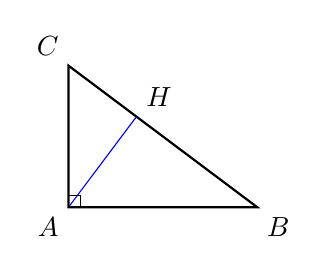
\begin{tikzpicture}[scale=0.6]
    \coordinate (A) at (0,0);
    \coordinate (B) at (4,0);
    \coordinate (C) at (0,3);
    \coordinate (H) at ($(B)!(A)!(C)$);
    
    \draw[thick] (A) -- (B) -- (C) -- cycle;
    \draw[blue] (A) -- (H);
    \draw (A) rectangle ++(0.25,0.25);
    
    \node[below left] at (A) {$A$};
    \node[below right] at (B) {$B$};
    \node[above left] at (C) {$C$};
    \node[above right] at (H) {$H$};
\end{tikzpicture}
\end{center}
\end{minipage}

\vspace{0.5em}

\question Đồ thị hàm số $y = (m-2)x + 3$ đi qua điểm $A(1; 5)$ khi $m$ bằng:
\begin{multicols}{4}
\begin{enumerate}[label=\Alph*.]
    \item $2$
    \item $4$
    \item $-2$
    \item $0$
\end{enumerate}
\end{multicols}

\question Đường tròn $(O; R)$ có bao nhiêu tiếp tuyến đi qua điểm $A$ nằm trên đường tròn?
\begin{multicols}{4}
\begin{enumerate}[label=\Alph*.]
    \item $0$
    \item $1$
    \item $2$
    \item Vô số
\end{enumerate}
\end{multicols}

\vspace{1em}
\hrule
\vspace{0.5em}

% ============================================================
% PHẦN TỰ LUẬN
% ============================================================
\textbf{II. PHẦN TỰ LUẬN} (6 điểm)

\vspace{0.5em}

\question \textbf{(2 điểm)} Cho đường tròn $(O; 5\text{cm})$. Từ điểm $A$ nằm ngoài đường tròn 
sao cho $OA = 13\text{cm}$, kẻ tiếp tuyến $AT$ với đường tròn ($T$ là tiếp điểm).

\begin{enumerate}[label=\alph*)]
    \item Tính độ dài đoạn tiếp tuyến $AT$.
    \item Tính diện tích tam giác $OAT$.
\end{enumerate}

\begin{center}
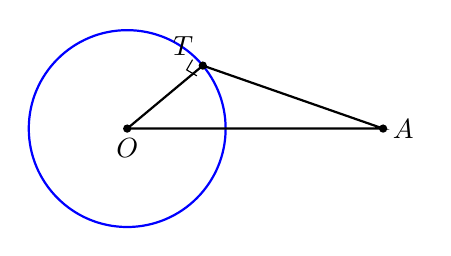
\begin{tikzpicture}[scale=0.5]
    \coordinate (O) at (0,0);
    \draw[thick, blue] (O) circle (2.5);
    
    \coordinate (A) at (6.5,0);
    \coordinate (T) at (1.92, 1.6);
    
    \draw[thick] (O) -- (T) -- (A) -- cycle;
    \draw (T) ++(150:0.3) -- ++(240:0.3) -- ++(330:0.3);
    
    \fill (O) circle (3pt);
    \fill (A) circle (3pt);
    \fill (T) circle (3pt);
    
    \node[below] at (O) {$O$};
    \node[right] at (A) {$A$};
    \node[above left] at (T) {$T$};
\end{tikzpicture}
\end{center}

\vspace{1em}

\question \textbf{(2 điểm)} Vẽ đồ thị hàm số $y = x^2$ và $y = 2x$ trên cùng hệ trục tọa độ. 
Tìm tọa độ giao điểm của hai đồ thị.

\begin{center}
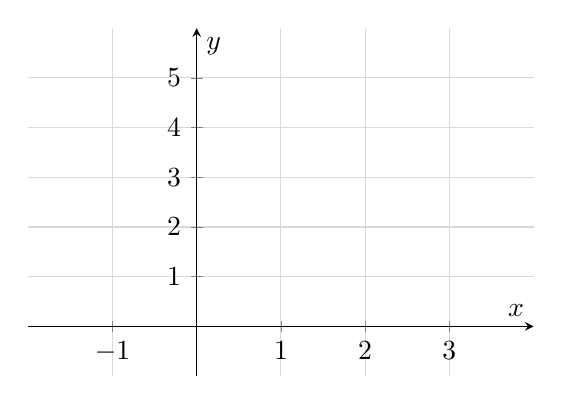
\begin{tikzpicture}
\begin{axis}[
    axis lines=middle,
    xlabel={$x$}, ylabel={$y$},
    xmin=-2, xmax=4,
    ymin=-1, ymax=6,
    grid=both,
    grid style={gray!30},
    width=8cm, height=6cm,
    xtick={-1,0,1,2,3},
    ytick={0,1,2,3,4,5},
]
    % Để trống cho học sinh vẽ
\end{axis}
\end{tikzpicture}
\end{center}

\vspace{1em}

\question \textbf{(2 điểm)} Cho tam giác $ABC$ có $AB = 6$, $AC = 8$, $BC = 10$.

\begin{enumerate}[label=\alph*)]
    \item Chứng minh tam giác $ABC$ vuông.
    \item Tính bán kính đường tròn ngoại tiếp tam giác $ABC$.
\end{enumerate}

% ============================================================
% FOOTER
% ============================================================
\vfill
\begin{center}
    \textbf{--- HẾT ---}
\end{center}

\end{document}
